The $\wmunuplusjets$ events can pass the SR selection in case the muon is
outside the detector acceptance or it fails quality criteria. This region
(CR$_\mathrm{\, wmn}$) thus selects $\wmunuplusjets$ events in order to estimate
the $\znunuplusjets$ contribution in the signal region. The muon is treated like
a neutrino in the $\met$ calculation, in this way the $W$ boson $\pt$ in this CR
is close to the $Z$ boson $\pt$ in $\znunuplusjets$ events in the SR\@. The
C$_{\mathrm{\, wmn}}$ region selects events with:
\begin{itemize}
\item Exactly one good muon.
\item The transverse mass, defined as:
  \begin{equation}
    \label{eq:82}
    m_\mathrm{\, T} = \sqrt{2 p_\mathrm{\, T}^{\, \mu} p_\mathrm{\, T}^{\, \nu}
      (1 - \cos(\phi_\mu - \phi_\nu))}
  \end{equation}
  and determined by the muon and neutrino $\pt$, is constrained in the
  $W$ boson mass window $30 < m_\mathrm{\, T} < 100$~GeV.
\end{itemize}
The transverse mass cut suppress the $\wtaunuplusjets$ processes in this
region. The measured $\met$ and leading jet $\pt$ distributions after the fit
procedure described in Section~\ref{sec:glob-simult-likel} are shown in
Figure~\ref{fig:muon_cr_plots}. The agreement between data and MC is good.

\begin{figure}[!h]
  \centering
  \begin{subfigure}[t]{.48\linewidth}
    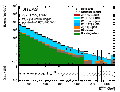
\includegraphics[width=\linewidth]{muon_cr_et_miss_post_fit}
    \caption{$\met$ distribution.}
    \label{fig:muon_cr_et_miss_pre_fit}
  \end{subfigure}
  \begin{subfigure}[t]{.48\linewidth}
    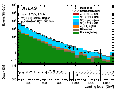
\includegraphics[width=\linewidth]{muon_cr_jet1_pt_post_fit}
    \caption{Leading jet $\pt$ distribution.}
    \label{fig:muon_cr_jet1_pt_pre_fit}
  \end{subfigure}
  \caption{Measured $\met$ and leading jet $\pt$ after fit distribution in the
    single muon CR for the $\met > 250~$GeV selection. The error bands include
    the statistical and systematic error.}
  \label{fig:muon_cr_plots}
\end{figure}
%%% Local Variables:
%%% mode: latex
%%% TeX-master: "../search_for_DM_LED_with_ATLAS"
%%% End:
